\chapter{The Detector}

\section{The Layout of CERN}

The Large Hadron Collider (LHC) is a 27-kilometer long proton-proton circular collider located underneath the border area of France and Switzerland, outside the city of Geneva. After accelerating protons to extremely high kinetic energies, the collider smashes two proton beams head-on at a center-of-mass energy of 13 TeV, converting the energy into mass and producing a spray of new particles. These collision events take place at four beam-crossing points located around the circumference of the accelerator ring, and the resulting data is captured by seven detectors. One of these detectors, ATLAS, is the focus of this study.

\section{An Anatomy of ATLAS}

The ATLAS detector (Figure~\ref{ATLAS}), built around one of the LHC beam crossing points, acts as a eight-story-tall recording device for measuring and digitizing the results of collisions. The detector contains multiple types of detection technology, each specialized to perform a specific type of measurement \cite{ATLAS_website}. The first major component of ATLAS is the inner detector. Composed of silicon pixel and strip detectors and transition radiation trackers, this portion of the detector is used to reconstruct the flight paths and momentums of charged particles. After this we have the electron calorimeter (ECAL), which captures and records the energies of electrons and photons through EM interactions. The hadronic calorimeter (HCAL) is after that, and being composed of heavy elements, it forces hadronic particles to deposit their energies through strong interactions. Finally, the detector is ringed by muon spectrometers, which detect the penetrating muons that pass unstopped through the rest of the detector. Neutrinos pass through ATLAS undetected, and their effects are seen in missing transverse momentum when the transverse momentums of all other decay products in the reaction are summed vectorially. These particle interactions are summed up in Figure~\ref{ATLAS}. Based on the hits recorded in a single collision, algorithms then reconstruct tracks, determine what particles were involved in the event, and figure out what happened in their brief lifetimes.
%A typical reconstructed event is shown in Figure~\ref{Higgs_2e2mu}. Here we see a Higgs boson decaying into two electrons and two muons. The muons, shown in red, pass through the detector, while the electrons shown in green deposit their energies in the ECAL. In this event, based on the energies of decay products, the original Higgs has been measured to have a mass of 122.6 GeV.

\begin{figure}[t]
    \centering
    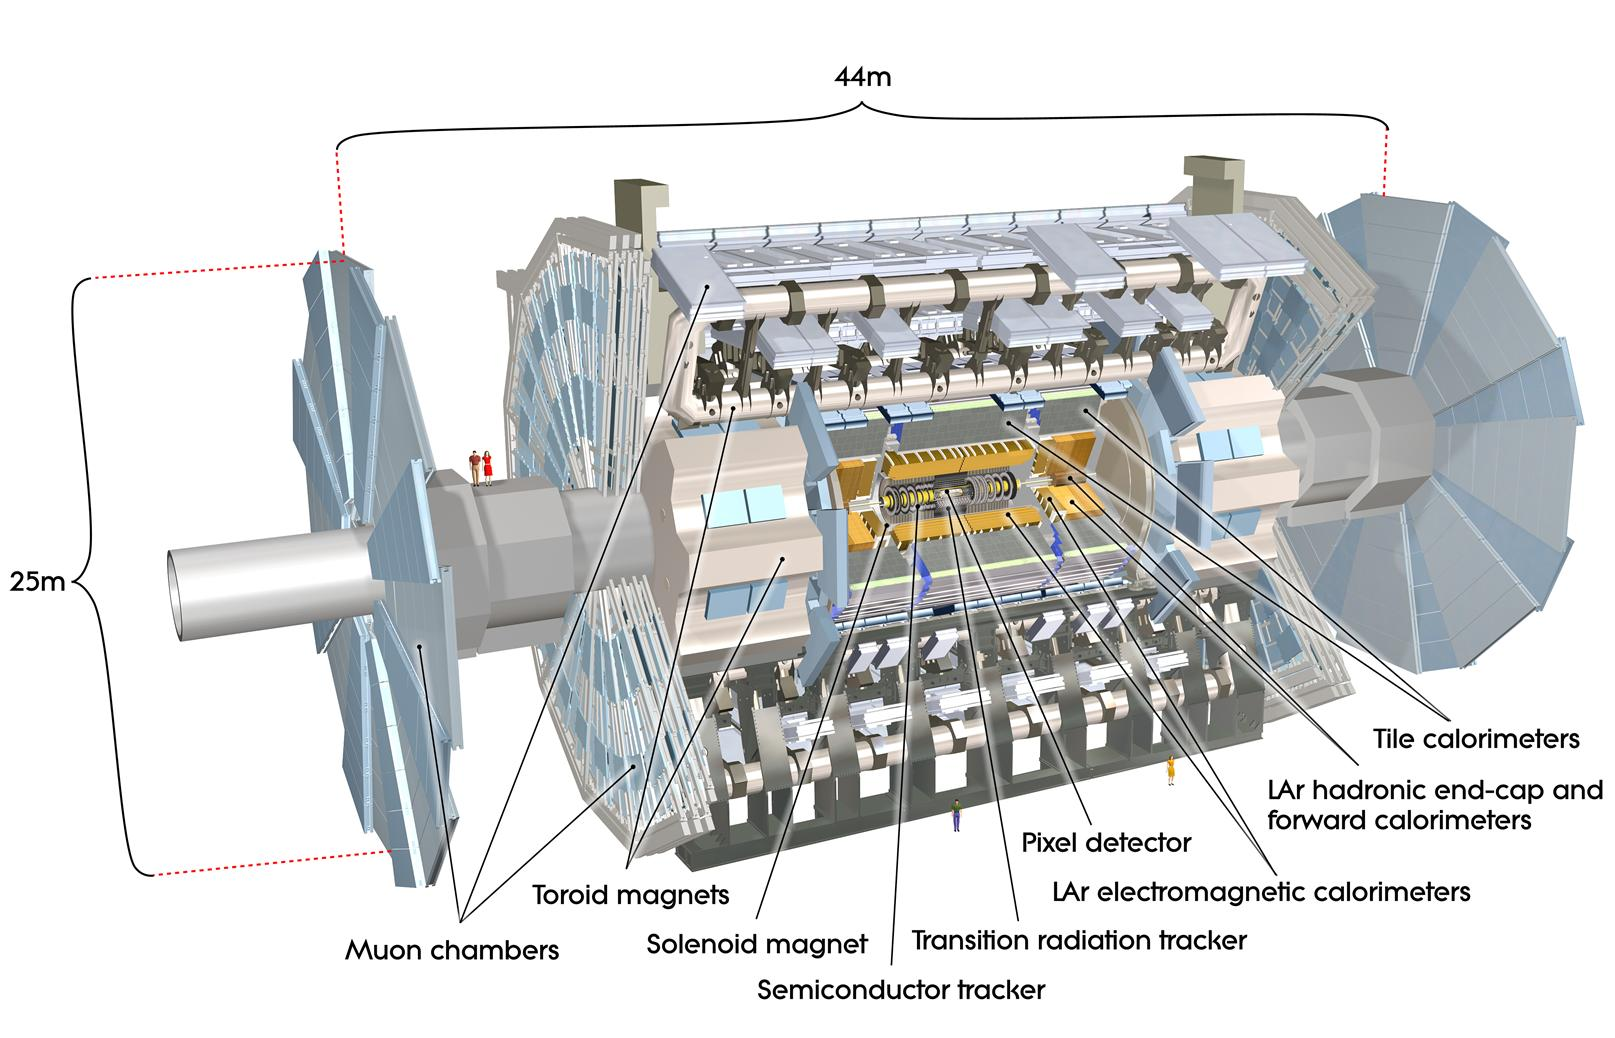
\includegraphics[width=0.49\linewidth]{images/ATLAS.png}
    \includegraphics[width=0.41\linewidth]{images/ATLASinteractions.jpg}
    \caption{(left) A labeled diagram of the ATLAS detector. (right) Interactions of different types of particles in ATLAS.}
    \label{ATLAS}
\end{figure}

%\begin{figure}[t]
%    \centering
%    \includegraphics[width=0.5\linewidth]{images/Higgs_2e2mu.png}
%    \caption{A typical reconstructed event display, showing a Higgs boson decaying into two electrons and two muons \cite{Higgs_2e2mu}.}
%    \label{Higgs_2e2mu}
%\end{figure}

\subsection*{Calorimeters}

%%%%%%%%%%%%%%%%%%%%%%%%%%%%%%%%%%%%%%%%%%%%%%%%%%%%%%%%%%%

The Large Hadron Collider (LHC) is a 27-kilometer long proton-proton circular collider located underneath the border area of France and Switzerland, outside the city of Geneva. After accelerating protons to extremely high kinetic energies, the collider smashes two proton beams head-on at a center-of-mass energy of 13 TeV, converting the energy into mass and producing a spray of new particles. These collision events take place at four beam-crossing points located around the circumference of the accelerator ring, and the resulting data is captured by seven detectors. One of these detectors, ATLAS, is the focus of this study.

The ATLAS detector (Figure~\ref{ATLAS}), built around one of the LHC beam crossing points, acts as a eight-story-tall recording device for measuring and digitizing the results of collisions. The detector contains multiple types of detection technology, each specialized to perform a specific type of measurement \cite{ATLAS_website}. The first major component of ATLAS is the inner detector. Composed of silicon pixel and strip detectors and transition radiation trackers, this portion of the detector is used to reconstruct the flight paths and momentums of charged particles. After this we have the electron calorimeter (ECAL), which captures and records the energies of electrons and photons through EM interactions. The hadronic calorimeter (HCAL) is after that, and being composed of heavy elements, it forces hadronic particles to deposit their energies through strong interactions. Finally, the detector is ringed by muon spectrometers, which detect the penetrating muons that pass unstopped through the rest of the detector. Neutrinos pass through ATLAS undetected, and their effects are seen in missing transverse momentum when the transverse momentums of all other decay products in the reaction are summed vectorially. These particle interactions are summed up in Figure~\ref{ATLAS}. Based on the hits recorded in a single collision, algorithms then reconstruct tracks, determine what particles were involved in the event, and figure out what happened in their brief lifetimes.
%A typical reconstructed event is shown in Figure~\ref{Higgs_2e2mu}. Here we see a Higgs boson decaying into two electrons and two muons. The muons, shown in red, pass through the detector, while the electrons shown in green deposit their energies in the ECAL. In this event, based on the energies of decay products, the original Higgs has been measured to have a mass of 122.6 GeV.

\begin{figure}[t]
    \centering
    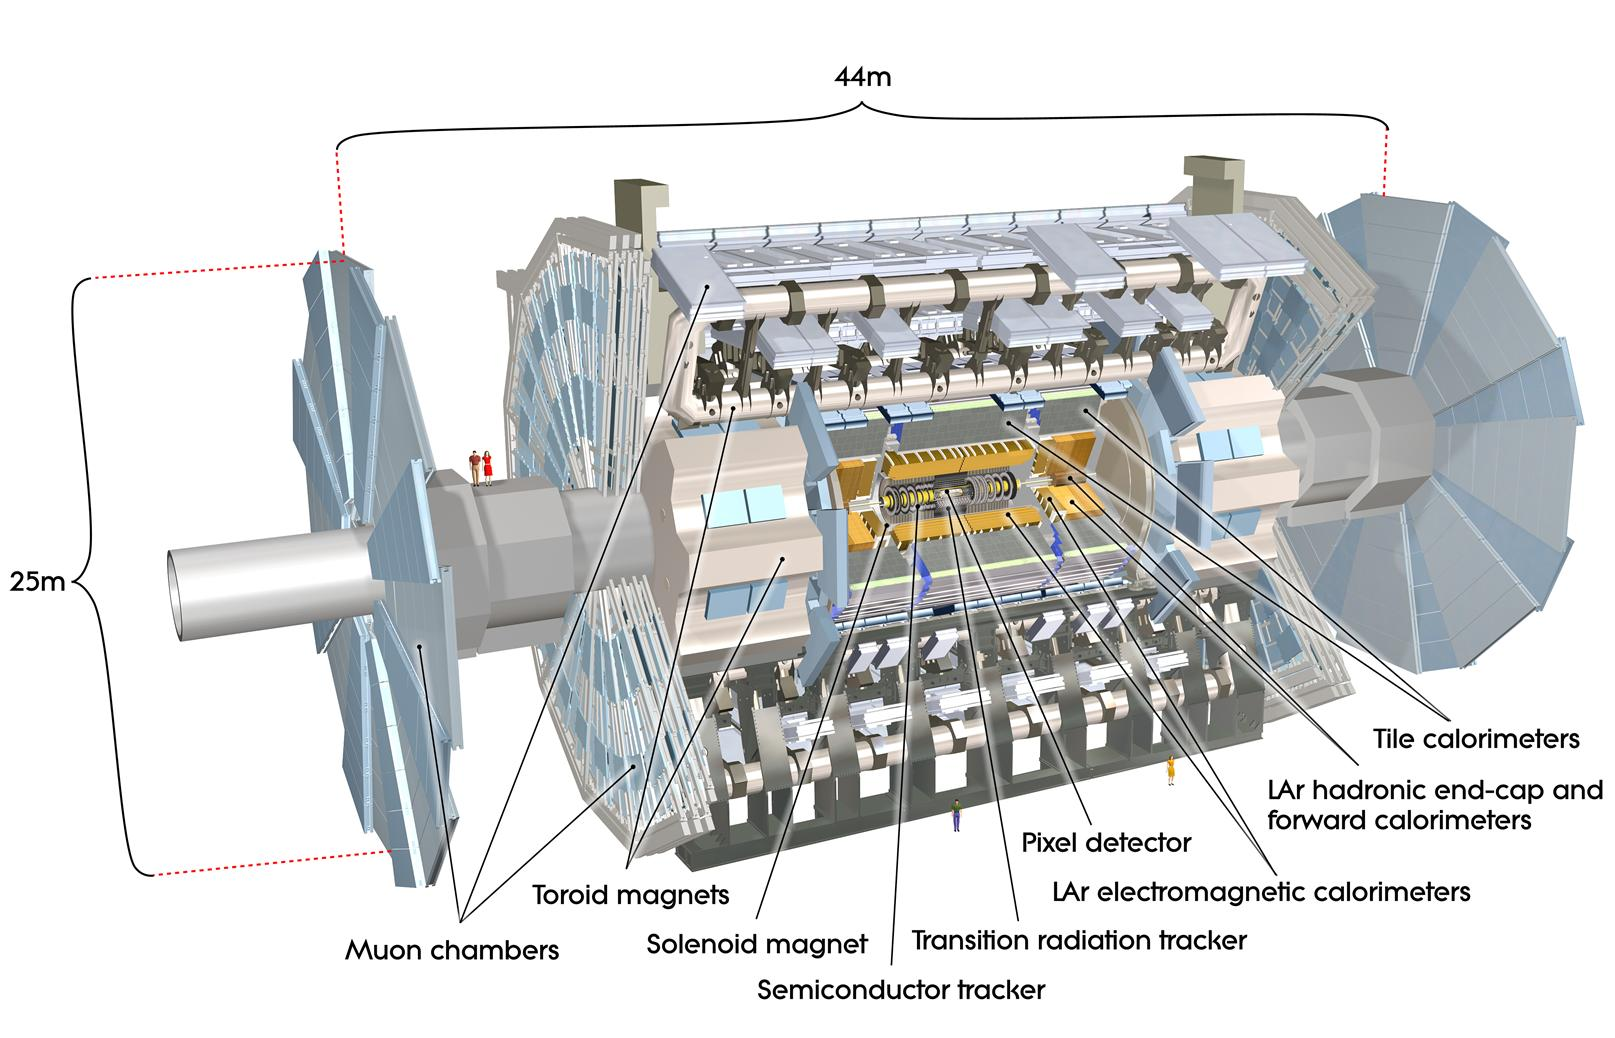
\includegraphics[width=0.49\linewidth]{images/ATLAS.png}
    \includegraphics[width=0.41\linewidth]{images/ATLASinteractions.jpg}
    \caption{(left) A labeled diagram of the ATLAS detector. (right) Interactions of different types of particles in ATLAS.}
    \label{ATLAS}
\end{figure}

%\begin{figure}[t]
%    \centering
%    \includegraphics[width=0.5\linewidth]{images/Higgs_2e2mu.png}
%    \caption{A typical reconstructed event display, showing a Higgs boson decaying into two electrons and two muons \cite{Higgs_2e2mu}.}
%    \label{Higgs_2e2mu}
%\end{figure}

\subsection*{Upgrades}

The LHC currently produces about 40 collisions per beam-crossing at 13 TeV center-of-mass energy, but with the proposed high-luminosity LHC (HL-LHC) upgrade there are plans to increase these numbers to 140 collisions per beam-crossing at 14 TeV by 2026, amounting to a total of 250 $fb^{-1}$ of data per year, with ultimate plans to increase to 200 collisions per beam-crossing. During the HL-LHC upgrade, ATLAS similarly plans to upgrade its detection capabilities via the ATLAS Phase-II upgrade, focusing on items such as replacing the inner detector with an all-silicon-based inner tracker (ITk), improving data acquisition, and increasing the granularity of calorimeters \cite{ATLAS_phaseII}. The higher data rates and improved calorimeters provide an incentive to develop and implement the machine-vision based particle identification systems described later in this paper. In the interest of improving upcoming SUSY searches, I have aided in the development of several components in the ATLAS detector. Though they will not be the focus of this paper, as they mostly impact future analyses, I would like to mention them in passing.

First, I worked on investigating methods for improving vertex reconstruction for use in future high-pileup environments, as part of the vertex reconstruction group at ATLAS. The approach we used was based on dividing physical space into a grid of three-dimensional pixels, and using reconstructed tracks to "fill in" those pixels and generate a 3D image. The resulting image was then Fourier transformed, filtered to remove high frequencies, reverse Fourier transformed, and collapsed along the beam axis, resulting in a 1D function where the peaks corresponded to potential vertex locations (vertex "seeds"). Tracks were then associated with their nearest seeds, and from each cluster of tracks we fit a final vertex. I performed performance comparisons between the new and old vertexing methods, and did studies based on tuning parameters of the new method. Some of these results were shown in my presentation at the 2015 ATLAS CP Tracking Workshop \cite{vertex}. I also performed studies on using machine-learning methods to better associate tracks with vertex seeds, and to recognize and recombine "split" vertices, though these methods did not show significant improvements over baseline during my time with the project.

I also performed some work on upgrades to the ITk for the ATLAS Phase-II upgrade. Recently I spent a year at Argonne under the guidance of Dr. Jessica Metcalfe working on manufacturing methods for mass production of silicon pixel detectors in preparation for the upgrade. During that time I worked on setting up a manufacturing lab and various electronic test environments, on assembling pixel modules using various mechanical epoxy-based techniques, on designing adapter boards for readout electronics, and on performing tests on assembled modules. I also participated in a three-month testbeam at Fermilab with the University of Geneva, during which we gathered and analyzed data from a proposed HVCMOS pixel detector. The idea behind this detector was that due to advances in silicon sensor manufacturing, we could build readout circuitry directly into the detector, removing the need for an external readout chip. This resulted in less detector material, and also reduced manufacturing cost. I presented results from this testbeam at DPF 2017 \cite{DPF}, and this analysis, combined with additional data taken by the University of Geneva at the SPS in CERN, will be presented in an upcoming paper on the new detector.

Furthermore, I have contributed some work to the fast tracker (FTk) upgrade for ATLAS \cite{FTk}. The FTk is an FPGA-based method for performing online track reconstruction, for use in the inner detector. I worked on the extrapolator board with Professor Mark Neubaeur's team. The extrapolator is responsible for reconstructing 12-layer tracks (for the 12 layers of the inner detector) using preliminary 8-layer tracks and a collection of hits from the other 4 layers. I developed a new memory storage mechanism for organizing and retrieving hits, and have recently completed a rewrite of the extrapolation code. We are currently working to ensure uninterrupted data flow, and are attempting to optimize our firmware to run at 200 MHz.